% LREC 2026 Example; 
% LREC Is now using templates similar to the ACL ones. 
\documentclass[10pt, a4paper]{article}

\usepackage{lrec2026}
\usepackage{cuted}
\usepackage{capt-of} 
\usepackage{graphicx}
\usepackage{fontspec}
\usepackage{array}
\usepackage{tabularx}
\usepackage{multirow}
\usepackage{hyperref}
\usepackage{booktabs}
\usepackage{tcolorbox}
\usepackage{subcaption} 
\newfontfamily\hindifont{Noto Sans Devanagari}[Script=Devanagari]% this is the new style
% the 'review' option anonymizes the paper following submission guideline
% the 'final' option produces the camera ready version (non anonymized)
% default version is 'final', so use review option for submission

\title{NeCCo: Nepali Cultural Commonsense Benchmark for Large Language Model Evaluation}

\name{Sanket Shrestha$^{*}$\thanks{$^{*}$Equal contribution}, 
Sadikshya Ghimire$^{*}$, 
Raunak Regmi$^{*}$,
Satyam Rana,
Supriya Khadka}

\address{Sunway College Kathmandu; Birmingham City University, Kathmandu, Nepal\\
         \{sanket\_24128469, sadikshya\_23140745, raunak\_regmi\_a25, satyam\_rana\_a25\, supriya\}@sunway.edu.np\\}



\abstract{
Large language models perform strongly on standard evaluations, yet these benchmarks prioritize high-resource languages and culturally dominant knowledge, leaving culture-specific commonsense underexamined. In low-resource languages such as Nepali, everyday communication depends on culturally embedded cues, including kinship hierarchies, ritual practices, food systems, idioms, and honorific distinctions that literal translation often fails to capture. As a result, models that appear competent on global metrics can perform poorly in local contexts. To address this gap, we introduce \textbf{NeCCo}, a curated multiple-choice benchmark for culturally situated reasoning across five domains: kinship and social hierarchy; festivals, rituals, and geography; idioms, proverbs, and metaphors; commonsense and daily life; and gastronomy, agriculture, and nature. The dataset was created through structured authoring, cross-review, and normalization, and is released in Devanagari, English, and Romanized formats. We evaluate multiple state-of-the-art LLMs using standardized prompting and controlled decoding. Results show substantial variation: models perform better on globally documented knowledge such as geography, but struggle with relational and linguistically implicit tasks, including extended kinship reasoning and proverb interpretation. The most culturally dense categories expose brittleness and increased hallucination. These findings suggest that multilingual competence requires more than translation coverage and highlight the need for culturally grounded benchmarks and training signals.
 \\ \newline \Keywords{{Cultural Common sense, Low-Resource Languages, Multilingual Evaluation, Benchmark Construction, LLM Evaluation, Cross-Cultural Reasoning.}} 
 }

\begin{document}


\maketitleabstract

\section{Introduction}
Nepali is an Indo-Aryan language spoken by over 17 million people and serves as the official language of Nepal. Despite its widespread use, it is considered a low-resource language in NLP due to its limited presence in large-scale training corpora and evaluation benchmarks \cite{shahi2022natural}. This under-representation leads to insufficient modeling of linguistic variability and culturally grounded nuances in large language models (LLMs) \cite{nyachhyon2025consolidating}. Many multilingual benchmarks either focus on high-resource languages or test translation-equivalent skills, which can obscure whether models actually understand locally grounded meanings in languages such as Nepali \cite{hu2020xtreme, liang2020xglue, nyachhyon2025consolidating}.

A key source of difficulty is cultural common sense: knowledge that speakers routinely use but rarely state explicitly. In Nepali, interpretation often depends on kinship structure and social hierarchy, honorific choice, ritual etiquette, and idiomatic language that does not survive literal translation \cite{krause1980kinship}. For example, kinship terms encode distinctions such as paternal versus maternal relations and elder versus younger relatives, and these distinctions shape appropriate address forms and expected behavior. Such cues are sparsely documented in globally available text and are therefore weakly represented in the data that dominates LLM training. As a result, a model can appear strong on general multilingual benchmarks while still failing on culturally specific reasoning required in everyday Nepali use \cite{thakur2025culturally}.

This paper targets that evaluation blind spot. We introduce NeCCo, a multiple-choice benchmark designed to test culturally anchored commonsense reasoning in Nepali across five domains: kinship and social hierarchy; festivals, rituals, and geography; idioms, proverbs, and metaphors; commonsense and daily life; and gastronomy, agriculture, and nature. We adopt a multiple-choice format to support controlled comparisons across models and prompt settings, reduce sensitivity to open-ended generation style, and enable fine-grained analysis of systematic confusions. At the same time, the format keeps the evaluation focused on selecting culturally appropriate inferences rather than on fluency or long-form explanation quality.

NeCCo is authored by native speakers and cross-reviewed to reduce ambiguity, with standardized formatting to support consistent evaluation. Using this benchmark, we evaluate a set of state-of-the-art LLMs under standardized prompting and decoding, and analyze performance by category to identify where culturally grounded reasoning breaks down \cite{thapa2025probing}. We then use these findings to highlight gaps in current multilingual evaluation practice and to motivate more culturally grounded training and assessment.

Our core contributions are
\begin{itemize}
    \item We introduce \textbf{NeCCo}, a culturally anchored multiple-choice benchmark for evaluating Nepali commonsense reasoning across five domains.
    \item We conduct a systematic evaluation of contemporary LLMs on culturally embedded reasoning tasks, highlighting failures that standard multilingual benchmarks can miss.
    \item We provide recommendations for future dataset construction and model training that incorporate culturally grounded signals.
\end{itemize}

\section{Related Work}


\subsection{Multilingual and Cross-Lingual Evaluation of LLMs}
A significant portion of LLM evaluation continues to rely on English-centric benchmarks. In these settings, multilingual capability is frequently inferred through translation or limited cross-lingual transfer rather than direct evaluation in the target languages~\cite{clark2020tydi}. Broad multilingual benchmarks, such as XTREME-style evaluation suites and information-seeking datasets like TyDi QA~\cite{clark2020tydi}, were introduced to assess generalization across typologically diverse languages. These evaluations consistently show significant performance degradation outside high-resource settings.

More recent evaluation frameworks, including holistic taxonomies and large collaborative benchmarks like BIG-bench~\cite{kazemi2025big}, emphasize the multi-dimensional nature of model quality. In these frameworks, aggregate accuracy can easily obscure failures in robustness, calibration, fairness, and cultural coverage. Multilingual extensions of complex reasoning benchmarks demonstrate that performance drops persist even under few-shot prompting. This indicates that multilinguality is not a uniform capability. Instead, it is a fragile interaction between training data distribution, script variation, and socio-cultural grounding~\cite{clark2020tydi}.

\subsection{Commonsense Reasoning Benchmarks}
Traditionally, commonsense reasoning benchmarks have focused on general-purpose inference, encompassing causal, temporal, physical, and social dimensions. However, widely used datasets such as CommonsenseQA, SocialIQA, and PIQA~\cite{sap2019social} are primarily constructed in English and implicitly encode Western or globally dominant knowledge priors~\cite{toroghi2025llm}. Cross-lingual efforts like XCOPA~\cite{ponti2020xcopa} reveal that transferring commonsense tasks across languages exposes distinct linguistic and cultural limitations. In many cases, translation-based approaches actually outperform direct multilingual reasoning~\cite{parashar2025inference}.

This highlights a major limitation: most existing benchmarks evaluate generalized commonsense rather than culturally situated reasoning. Key dimensions like kinship structures, honorific systems, ritual practices, and idiomatic expressions remain starkly underrepresented. This creates a critical evaluation gap where models appear competent in abstract reasoning but fail in culturally grounded contexts.

\subsection{Cultural and Socio-Cultural Bias in LLMs}

A parallel body of work investigates cultural and socio-cultural bias in LLMs, demonstrating that models inherently encode and reproduce patterns present in their training data. Foundational benchmarks such as CrowS-Pairs~\cite{nangia2020crows} and StereoSet~\cite{nadeem2021stereoset} measure stereotypical associations, BBQ~\cite{parrish2022bbq} evaluates bias in question answering, and HolisticBias~\cite{zake2023holistic} expands this coverage across multiple demographic dimensions. Although essential for assessing fairness, these tools are largely centered on English-speaking or Western contexts. This geographical and linguistic concentration leaves significant gaps in understanding localized harms, such as the specific mechanisms of gender bias in under-represented languages like Nepali~\cite{khadka2025gender}. Emerging work on culturally diverse evaluation highlights that true cultural competence extends beyond simple bias mitigation. It requires a nuanced understanding of implicit norms, localized knowledge systems, and culturally bounded meanings~\cite{piaobeyond}. When confronted with unfamiliar cultural inputs in these settings, LLMs frequently exhibit hallucination, over-generalization, or default to globally dominant interpretations~\cite{peters2022generalization}.

\subsection{Low-Resource and Nepali NLP}

Low-resource languages present a unique set of challenges characterized by limited high-quality corpora, sparse benchmark availability, and severe under-representation in large-scale training pipelines. Nepali exemplifies this pattern: despite being spoken by millions, it remains critically under-resourced in terms of standardized evaluation frameworks~\cite{cahyawijaya2024llm}. Existing efforts in Nepali NLP have primarily focused on foundational tasks, including part-of-speech tagging~\cite{pradhan2024parts}, named entity recognition~\cite{singh2019named}, machine translation~\cite{shahi2022natural}, text classification~\cite{prabha2018deep} and text-to-speech~\cite{khadka2023tts}. Benchmarks such as Nep-gLUE~\cite{timilsina2022nepberta} and subsequent Nepali NLU datasets~\cite{nyachhyon2025consolidating} have contributed to task-level standardization. Concurrently, monolingual models like NepBERTa have demonstrated improved performance over multilingual baselines in specific settings~\cite{timilsina2022nepberta}. Additionally, resources such as FLoRes provide reliable evaluation datasets for Nepali in machine translation~\cite{guzman2019flores}. However, these efforts largely target conventional syntactic or semantic tasks. Much of Nepali reasoning is transmitted through oral tradition and lived experience rather than formal corpora, making it particularly difficult for models to learn through these standard, foundational training datasets.

\subsection{Toward Culturally Grounded Evaluation}

Recent work has increasingly highlighted the limitations of large language models in capturing culturally grounded reasoning, particularly beyond high-resource and globally dominant contexts. While several benchmarks have been proposed for South Asian languages, most focus on broader Indic settings or emphasize translation-based evaluation rather than culturally embedded understanding. Datasets such as SANSKRITI ~\cite{maji2025sanskriti} and MILU ~\cite{verma2025milu} evaluate LLMs across multiple Indic languages and domains, demonstrating that model performance drops in culturally rich categories such as rituals, social norms, and traditional knowledge~\cite{joshi2025elr}. Similarly, large-scale multilingual evaluations like PARIKSHA reveal inconsistencies and reduced reliability of LLMs in low-resource languages, particularly when tasks require implicit reasoning or contextual awareness. However, these efforts largely aggregate across languages and do not account for the unique sociocultural structures of individual languages such as Nepali, as cultural common-sense in Nepali remains underrepresented in existing benchmarks. ~\cite{chiu2025culturalbenchrobustdiversechallenging}.

\section{Methodology}

\subsection{Dataset Creation}

The Nepali Cultural \& Commonsense Benchmark (\textbf{NeCCo}) is a curated dataset of 1,295 four-option multiple-choice questions (A--D) designed to evaluate culturally grounded reasoning in Nepali.\footnote{NeCCo is publicly available at \url{https://github.com/Mezamenta-Nakama09/NeCCo}.} Each question has a single correct answer, and the distractors are written to be plausible without requiring external tools or specialized knowledge.

To study script sensitivity and translation, each question is released in aligned Devanagari Nepali and Romanized Nepali. Romanized Nepali refers to the phonetic transcription of the native Devanagari script into the Latin alphabet, a format widely used in informal digital communication~\cite{madhani2023aksharantar}. Unlike standard Devanagari, Romanized text often lacks rigid spelling conventions. For example, the Devanagari word {\hindifont `राम्रो'} (good) is commonly romanized as `'\textit{ramro}', and a phrase like {\hindifont `के छ?'} (What's up?) might appear variously as \textit{`ke cha'}, \textit{`k cha'}, or \textit{`k chha'}.

We additionally provide English translations for categories where translation does not substantially distort the intended reasoning signal. Accordingly, the \textit{Kinship \& Social Hierarchy} and \textit{Idioms, Proverbs \& Metaphors} categories do not include English translations to preserve nuance. In total, NeCCo contains 3,460 released items: 1,295 (Devanagari) + 1,295 (Romanized) + 870 (English).\footnote{The 870 English items correspond to the 1,295 total questions minus the 425 questions in the two non-translated categories.} Category counts are shown in Table~\ref{tab:data_category_count}.

\begin{table}[h]
    \centering
    \small
    \begin{tabular}{lc}
    \hline
    \textbf{Category} & \textbf{Questions} \\
    \hline
    Kinship \& Social Hierarchy            & 235 \\
    Festivals, Rituals \& Geography        & 382 \\
    Idioms, Proverbs \& Metaphors          & 190 \\
    Commonsense \& Daily Life              & 200 \\
    Gastronomy, Agriculture \& Nature      & 288 \\
    \hline
    \end{tabular}
    \caption{\small Number of questions per category in NeCCo.}
    \label{tab:data_category_count}
\end{table}

\paragraph{Category Design}
NeCCo is organized into five categories chosen to reflect dimensions of Nepali cultural knowledge and everyday reasoning:

\begin{itemize}
    \item \textbf{Kinship \& Social Hierarchy:} Tests understanding of kinship terms and social relations that encode lineage (maternal vs.\ paternal), birth order, and marital ties, as well as associated expectations of respect and address.
    \item \textbf{Festivals, Rituals \& Geography:} Covers religious and cultural observances, ritual objects and practices, and region-specific events shaped by Nepal’s geography.
    \item \textbf{Idioms, Proverbs \& Metaphors:} Focuses on culturally embedded expressions whose meanings cannot be derived from literal translation, requiring contextual interpretation.
    \item \textbf{Commonsense \& Daily Life:} Targets implicit norms in daily interactions, including etiquette, hospitality, purity concepts, and socially appropriate behavior.
    \item \textbf{Gastronomy, Agriculture \& Nature:} Grounded in culinary practice and agrarian routines, like ingredient pairings, seasonality, planting cycles, and common tools.
\end{itemize}

Representative examples from each category and each released variant are provided in Appendix~\hyperref[app:examples]{A}.

\paragraph{Data Collection and Validation}
All four authors are native Nepali speakers and collaboratively developed the dataset. Each author led one or two categories to ensure domain focus while maintaining coverage diversity. Questions were primarily sourced from shared community knowledge and lived cultural experience, with attention to regional and ethnic variation.

We used a multi-stage validation pipeline. After initial authoring, question sets were exchanged for peer review. Reviewers labeled each item as \textit{Keep}, \textit{Modify}, or \textit{Delete} based on cultural accuracy, ambiguity, distractor plausibility, and clarity. Items marked \textit{Modify} were revised iteratively, and disputed cases were resolved through discussion until consensus.

\paragraph{Cleaning, Translation and Alignment}
After review, we manually corrected spelling, grammar, and factual issues. We also applied automated checks for duplicates, missing fields, CSV formatting consistency, and ID sequencing.

For the categories that include English, we generated initial translations using Google Translate\footnote{\href{https://translate.google.com/}{https://translate.google.com/}} and then refined them with bilingual native speakers to preserve meaning. Romanization was standardized across entries. Finally, we performed cross-checks to ensure consistent alignment across Devanagari, Romanized Nepali, and English variants.

\subsection{Experimental Setup}

\subsubsection{LLMs Used}
We evaluate nine recent LLMs chosen to span a range of architectures, release types (proprietary vs.\ open-weight), and multilingual capabilities. Model selection was informed by contemporaneous standings on OpenRouter and other public leaderboards, with an emphasis on general instruction following and multilingual reasoning performance at the time of evaluation.\footnote{\href{https://openrouter.ai/rankings}{https://openrouter.ai/rankings}}

The evaluated models are: GPT-4o-mini, GPT-5.2, and GPT-OSS-120B (OpenAI) \cite{hesham2024finetuning, ma2026safetyreport, openai2025gptoss}; Gemini 3 Flash Preview (Google DeepMind) \cite{zhang2026ophthalmology}; DeepSeek V3.2 \cite{deepseek2025v3}; Grok 4.1 Fast (xAI) \cite{ma2026safetyreport}; GLM-5 (Tsinghua University and Zhipu AI) \cite{zeng2026glm5}; Minimax M2.5 \cite{ko2026bilingualbias}; and Trinity Large Preview \cite{openrouter2026}. We include Trinity Large Preview in particular because it accounts for the highest usage share for Nepali on OpenRouter (see Appendix~\hyperref[app:openrouter_trinity]{C}), making it a highly relevant, community-preferred baseline for culturally grounded Nepali evaluation.

\begin{figure*}[htbp]
    \centering
    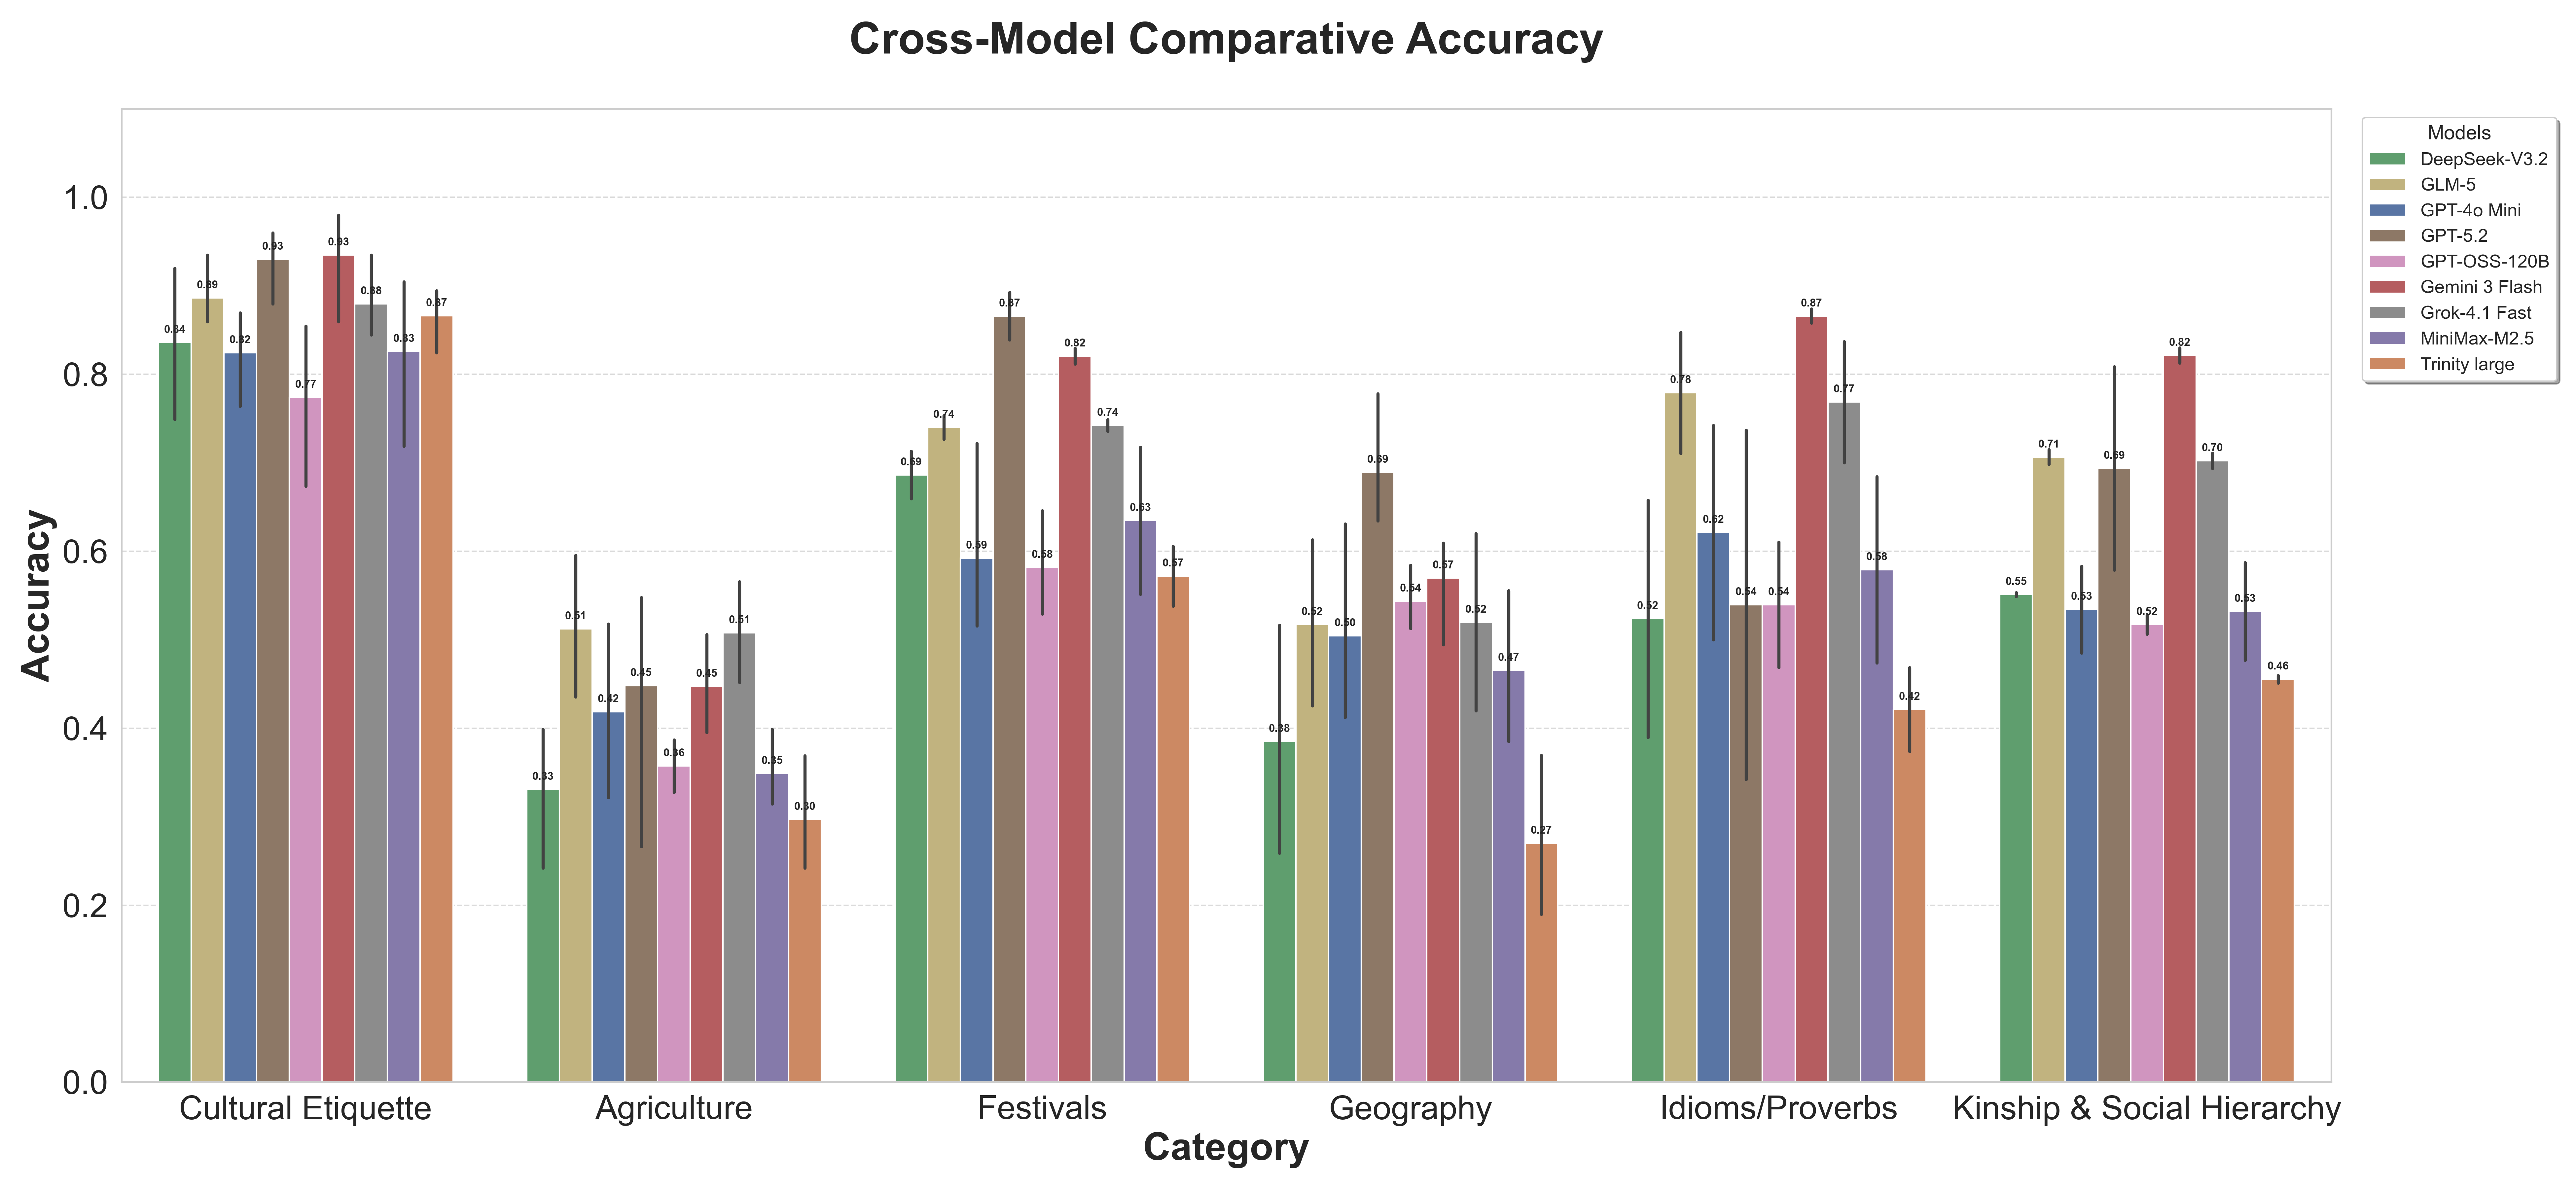
\includegraphics[width=\textwidth]{benchmark_bar_chart.png}
    \caption{Comparative Accuracy across Categories}
    \label{fig:benchmark_bar_chart}
\end{figure*}

\subsubsection{Evaluation Procedure}
We use a standardized few-shot prompting setup (2-shot) for all models. Two fixed example question-answer pairs are prepended to every evaluation instance across all categories. Keeping the demonstrations and instructions constant ensures that performance differences primarily reflect the model’s reasoning, rather than variation in prompt framing. The prompt template and demonstrations are shown Figure~\ref{fig:prompt_template}.

\begin{figure}
\begin{tcolorbox}[
    colback=gray!5!white,
    colframe=gray!75!black,
    title=Prompt Format (2-shot MCQ),
    boxrule=0.8pt,
    arc=2pt,
    left=6pt,
    right=6pt,
    top=6pt,
    bottom=6pt
  ]
  \textbf{System/Instruction:} You are a helpful assistant that answers multiple choice questions about Nepali common sense and cultural etiquette. Your task is to provide ONLY the letter (A, B, C, or D) corresponding to the correct option. Do NOT provide any reasoning, explanation, or additional text. Just the single letter.
  
  \vspace{0.5em}
  \textbf{Example 1:}\\
  \textbf{Question:} {\hindifont तिमी आफन्तको घरमा खाना खाँदै छौ। काँक्रोको अचार एकदम पिरो छ। चलन अनुसार तिमीले के गर्छौ?}\\
  \textbf{A:} {\hindifont मुखबाट 'आफ्, आफ्' आवाज निकाल्दै पानी माग्छौ।}\\
  \textbf{B:} {\hindifont थोरै भात वा चिउरासँग मुछेर चुपचाप निल्छौ।}\\
  \textbf{C:} {\hindifont अचारलाई थालको छेउमा थुक्छौ।}\\
  \textbf{D:} {\hindifont पाहुनालाई गाली गर्छौ।}\\
  \textbf{Answer:} B
  
  \vspace{0.5em}
  \textbf{Example 2:}\\
  \textbf{Question:} {\hindifont तिमी मन्दिर भित्र छौ। देउतालाई ढोग्दा तिम्रो टाउकोले केमा छुने कोसिस गर्छौ?}\\
  \textbf{A:} {\hindifont मन्दिरको सिँढीमा।}\\
  \textbf{B:} {\hindifont देउताको पाउ वा तोकिएको चरण-पादुकामा।}\\
  \textbf{C:} {\hindifont घण्टीमा।}\\
  \textbf{D:} {\hindifont पुजारीको हातमा।}\\
  \textbf{Answer:} B
  
  \vspace{0.5em}
  \textbf{Evaluation Instance Template:}\\
  \textbf{Question:} \{question\}\\
  \textbf{A:} \{A\}\\
  \textbf{B:} \{B\}\\
  \textbf{C:} \{C\}\\
  \textbf{D:} \{D\}\\
  \textbf{Answer:}
\end{tcolorbox}
\caption{Prompt Template}
\label{fig:prompt_template}
\end{figure}

All models are evaluated on the same four-way MCQ task and are instructed to output \emph{only} the option letter. We use a uniform system prompt and identical input formatting for all models to minimize differences due to verbosity, output style, or prompt interpretation, and to focus the evaluation on answer selection.

Inputs are evaluated in three representations: Devanagari Nepali, Romanized Nepali, and English translation (except for the two categories where English is intentionally omitted). All models are accessed through a unified API interface. Decoding settings are kept consistent across models by using a single set of parameters, with no model-specific tuning. Each question is submitted exactly once per model and representation, with no resampling or response averaging. Outputs are logged automatically to CSV along with the gold label, predicted option, and an automatically computed correctness field.


\begin{figure*}[t]
    \centering
    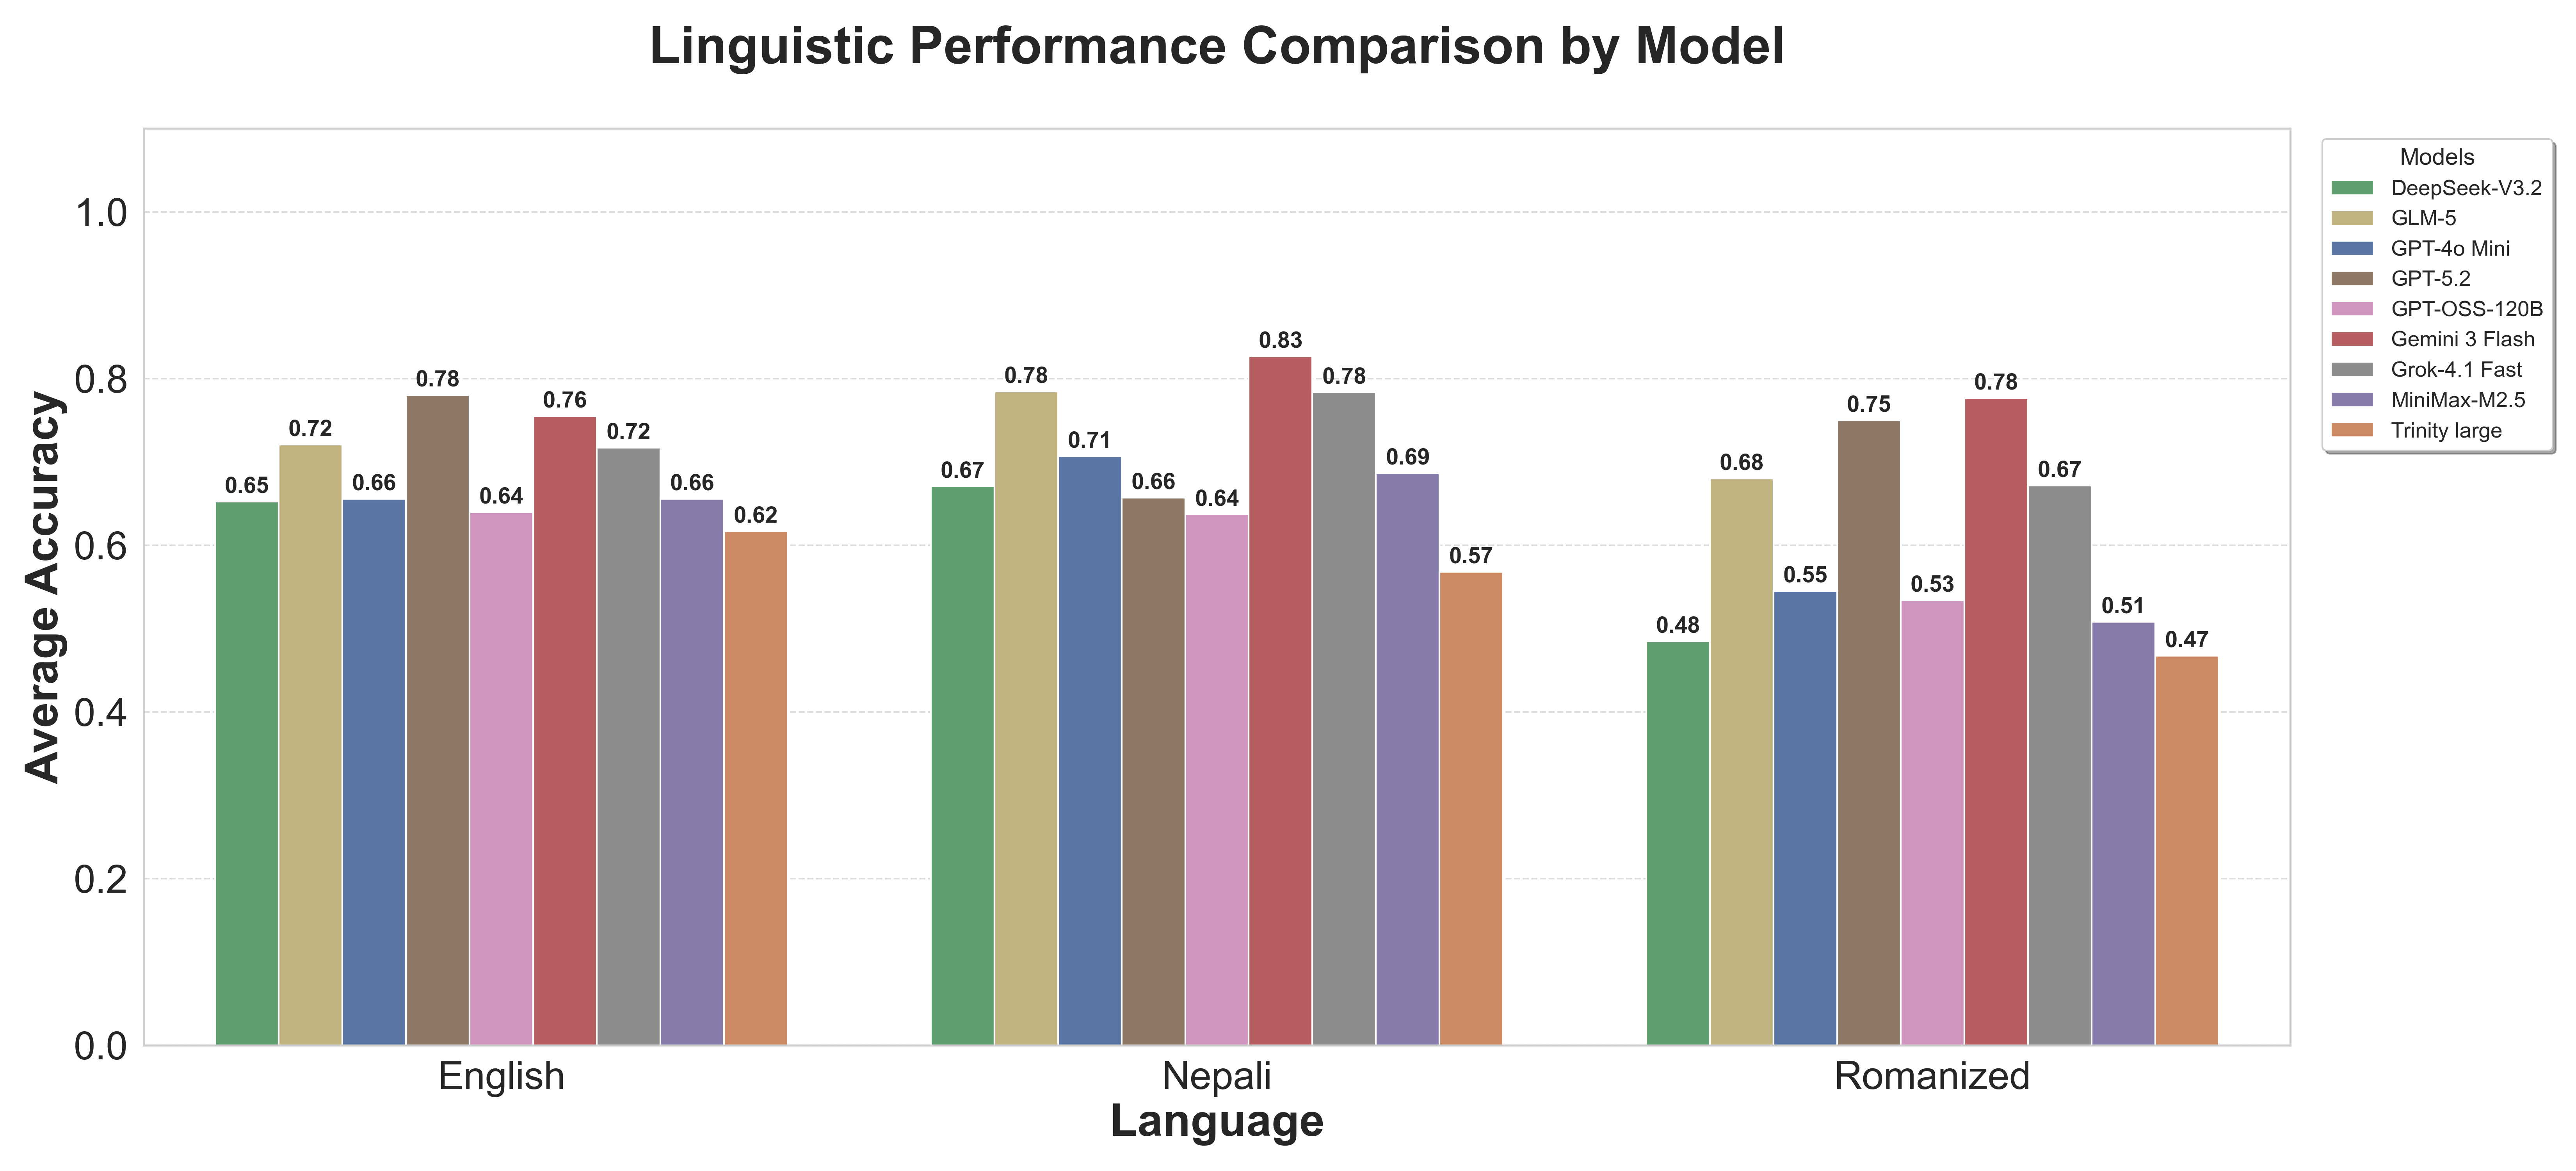
\includegraphics[width=\textwidth]{language_comparison_bar.png}
    \caption{Performance Comparison: English vs. Nepali vs. Romanized}
    \label{fig:language_comparison_bar}
\end{figure*}


\subsubsection{Analysis Protocol}
We evaluate model performance using \textbf{accuracy}, measured as the proportion of questions for which a model selects the correct option. Beyond overall accuracy, we report results \textbf{by category} to better capture domain-specific strengths and weaknesses, since aggregate scores can mask substantial variation across cultural domains.

We further stratify performance across the three input representations: \textbf{Devanagari Nepali}, \textbf{Romanized Nepali}, and \textbf{English translation}. This breakdown enables a direct assessment of how sensitive models are to changes in script and language form. For culturally dense categories such as \textit{Kinship \& Social Hierarchy} and \textit{Idioms, Proverbs \& Metaphors}, we do not include English-based analysis because English translations were intentionally omitted to avoid loss of meaning and evaluation ambiguity.

Finally, we compare performance across models, categories, and representations to identify recurring error patterns and question types that are systematically challenging. Although our primary metric is accuracy, these structured slices provide a clearer view of model limitations and highlight where cultural knowledge and language representation most strongly influence performance.

\begin{figure*}[t]
    \centering

    \begin{subfigure}[t]{0.45\textwidth}
        \centering
        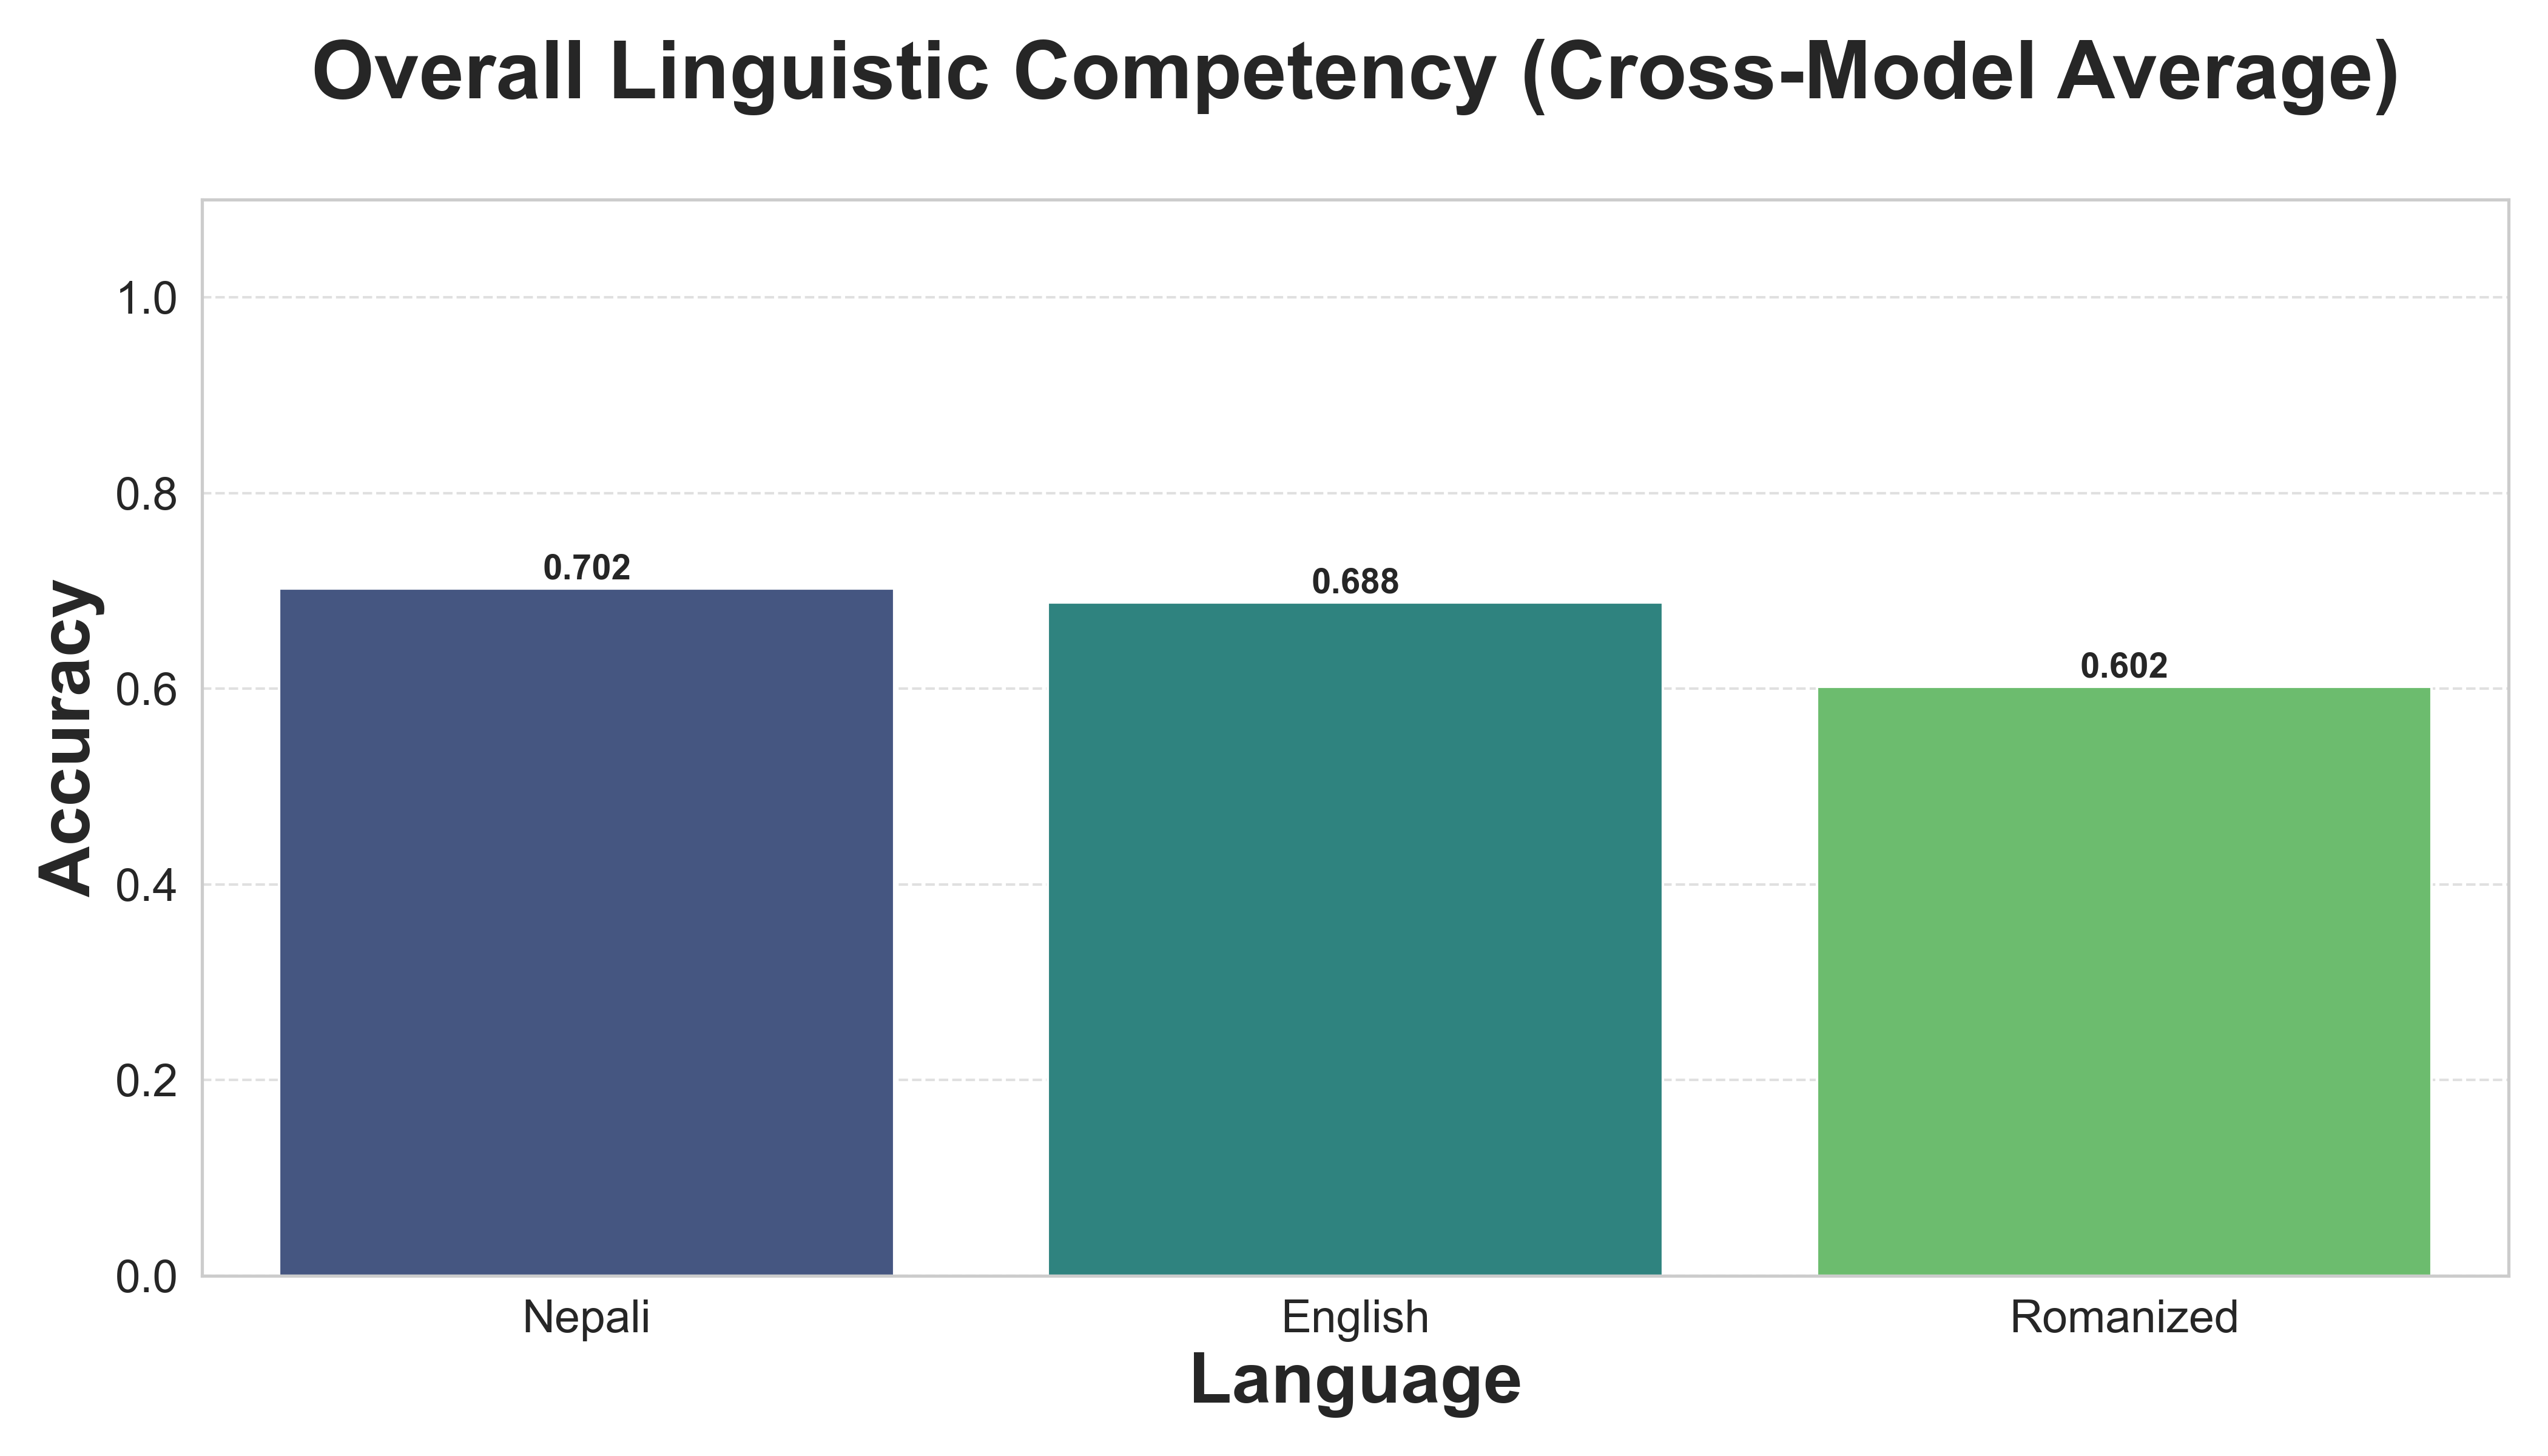
\includegraphics[width=\textwidth]{overall_language_performance.png}
        \caption{Overall Language Performance Across All Models}
        \label{fig:overall_language_performance}
    \end{subfigure}
    \hfill
    \begin{subfigure}[t]{0.49\textwidth}
        \centering
        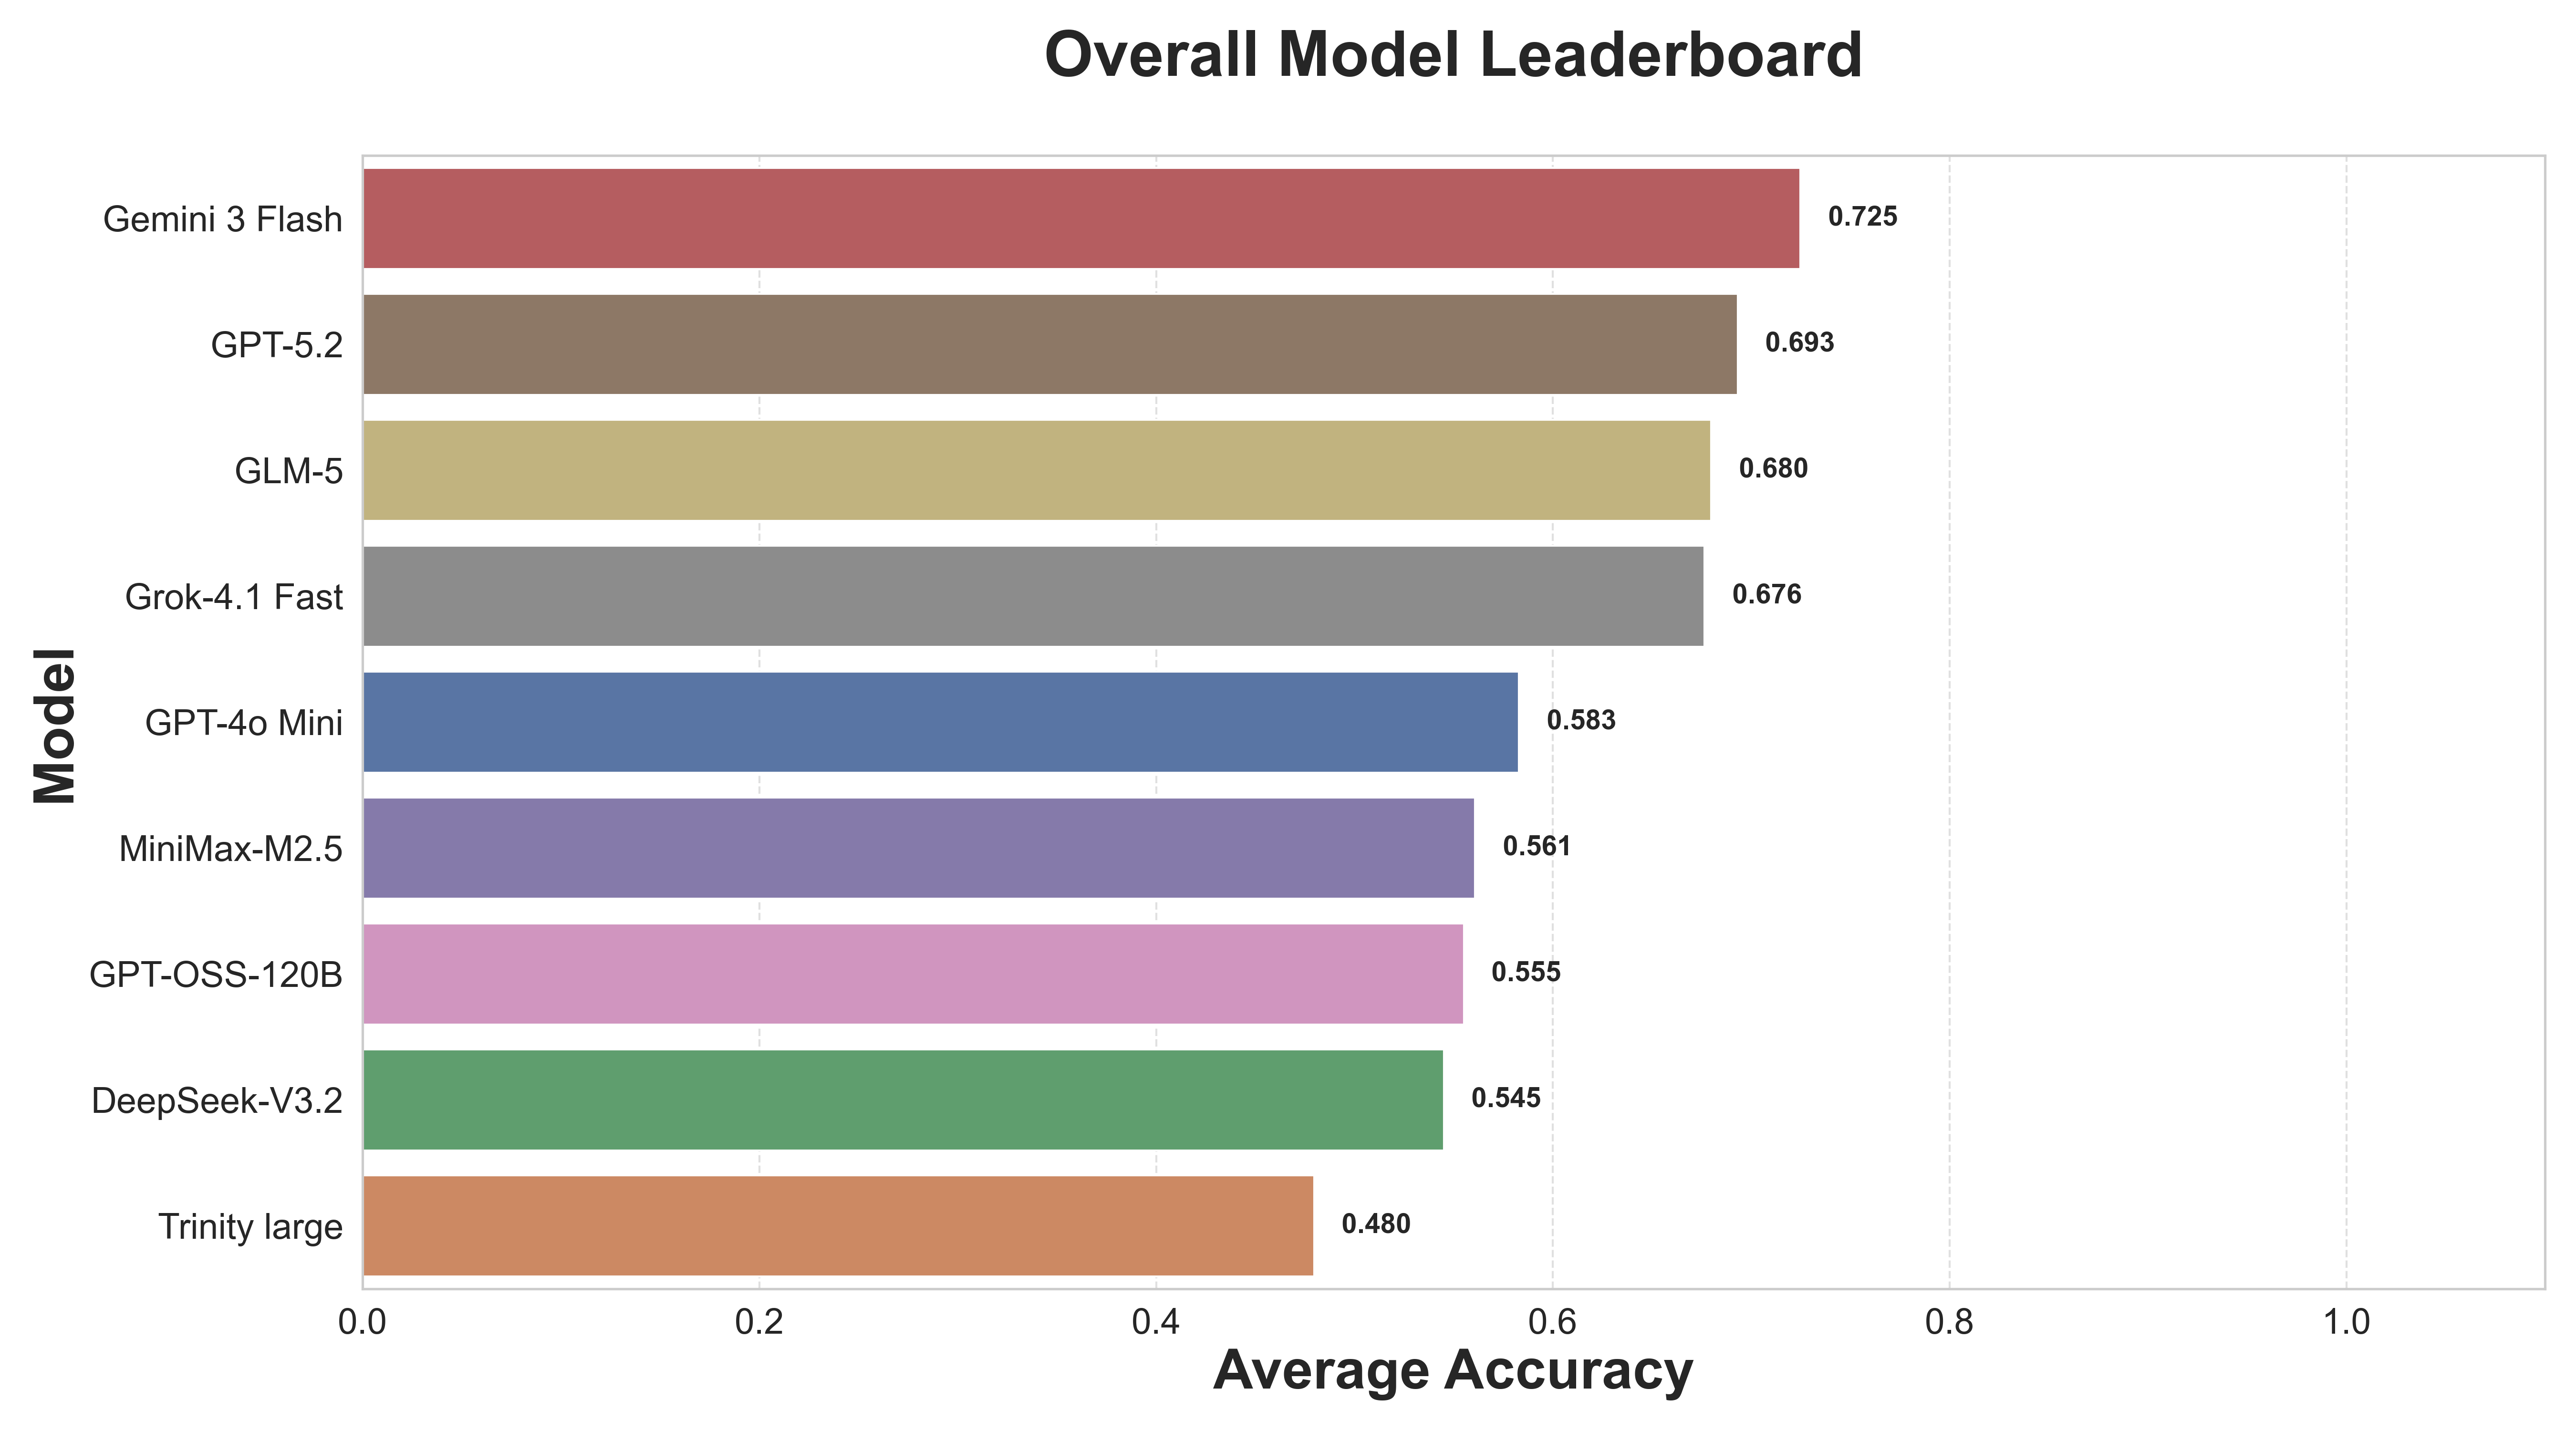
\includegraphics[width=\textwidth]{overall_ranking.png}
        \caption{Overall Model Ranking (Mean Accuracy Across All Categories)}
        \label{fig:overall_ranking}
    \end{subfigure}

    \caption{Aggregate results across input representations and models.}
    \label{fig:overall_language_and_ranking}
\end{figure*}

\section{Results}
In this section, we summarize overall trends in accuracy to highlight where current LLMs succeed and where they systematically fail on Nepali cultural commonsense. A complete breakdown of per-model results, including accuracy, precision, recall, and F1 across categories and representations, is provided in the Appendix~\hyperref[app:full_results]{B}.

\paragraph{Comparative Accuracy across Categories. }
Figure~\ref{fig:benchmark_bar_chart} illustrates a significant imbalance in how models capture cultural knowledge across different domains. Models perform exceptionally well on widely documented domains. For instance, Cultural Etiquette is the best performing category, with both GPT-5.2 and Gemini 3 Flash achieving peak accuracies of 0.93. Festivals also demonstrate strong cross-model performance, with top models consistently scoring above 0.80.

Conversely, performance drops sharply on localized, community-specific domains like Agriculture and Geography. Agriculture is the most universally challenging category. Even the highest-performing models struggle in this area, with scores hovering between 0.30 and 0.51. This suggests a widespread deficit in implicit or rural localized knowledge. Furthermore, categories like Idioms/Proverbs and Kinship \& Social Hierarchy are highly model-dependent. Gemini 3 Flash excels in Idioms/Proverbs (0.87) and Kinship (0.82), whereas models like Trinity large and DeepSeek-V3.2 struggle significantly in these exact same categories (scoring between 0.42 and 0.55). This variance indicates that specific training mixtures allow certain models to grasp complex linguistic and social nuances that others miss. 

\paragraph{Performance Comparison: English vs. Nepali vs. Romanized. }
Figure~\ref{fig:language_comparison_bar} isolates the role of script and language form by evaluating each question across three formats. While aggregate trends favor native script, individual models exhibit fascinating divergence in their linguistic handling. Models such as Gemini 3 Flash and GLM-5 perform best in native Devanagari (0.83 and 0.78 respectively), outperforming their own English baselines. However, this is not a universal rule. GPT-5.2 demonstrates an inverted proficiency, performing best in English (0.78), followed by Romanized Nepali (0.75), and performing worst in native Devanagari (0.66). A similar trend is visible with GPT-4o Mini. This highlights that multilingual alignment varies heavily by model architecture, and language representation choices materially affect how reliably cultural commonsense is retrieved.

\paragraph{Overall Language Performance Across All Models. }
Figure~\ref{fig:overall_language_performance} consolidates the linguistic results across all models to confirm a stable overall ordering. Native Devanagari Nepali achieves the highest aggregate accuracy (0.702), followed closely by English (0.688). Romanized Nepali represents a significant step down (0.602). This aggregate pattern suggests that non-standard transliteration meaningfully hinders an LLM's access to its culturally grounded knowledge base.

\paragraph{Overall Model Ranking.}
Finally, Figure~\ref{fig:overall_ranking} presents the overall leaderboard, revealing a distinct stratification in model capabilities. The top tier of models demonstrates a clear advantage, with Gemini 3 Flash leading the benchmark at an average accuracy of 0.725. This is followed closely by GPT-5.2 (0.693), GLM-5 (0.680), and Grok-4.1 Fast (0.676). There is a notable drop-off to the second tier of models, beginning with GPT-4o Mini (0.583) and cascading down to Trinity large (0.480). This distribution indicates that larger parameter counts or general popularity do not automatically guarantee superior cultural reasoning, as highly optimized models often outperform larger alternatives.

\section{Discussion}
The NeCCo evaluation offers a detailed view of how well current LLMs capture Nepali cultural intelligence. While the top-performing systems show strong general capabilities, we observe recurring failure modes that expose the limits of today's models in culturally grounded commonsense reasoning. In many cases, models handle surface-level facts and linguistic form reliably but struggle when correct answers depend on implicit norms, context-specific practices, or culturally encoded meanings that native speakers take for granted.

\subsection{The Importance of Cultural Benchmarking}
Most standard NLP benchmarks emphasize linguistic competence, general knowledge, or skills that transfer well across languages. They rarely test the everyday commonsense and social expectations that are obvious within a community but opaque to outsiders. NeCCo illustrates why culturally targeted benchmarks are necessary: models can appear highly capable on global tasks while still failing in realistic local scenarios where appropriate behavior, social roles, and cultural interpretations matter.

This has practical implications for deployment. A model may produce fluent Nepali and handle translation accurately, yet remain unreliable when advising users in culturally sensitive contexts such as kinship address terms, social hierarchy, ritual practices, or community norms. Evaluating these dimensions helps prevent a form of cultural erasure in which systems are treated as ``Nepali-capable'' based primarily on language form, even though they lack key cultural competencies required for safe and useful real-world interaction.

Our results also underscore that cultural understanding does not automatically transfer through translation. The performance gap between English and Devanagari Nepali suggests that knowing a concept in English is not the same as recognizing its lived meaning, associated norms, and situational usage in Nepali contexts. Cultural competence therefore requires more than mapping words across languages. It requires interpreting meaning within local practices, expectations, and history.

\subsection{Key Findings and Observations}

\paragraph{Linguistic Representation and Script Sensitivity}
A consistent pattern in our findings is the clear advantage of native-script inputs. For several top-tier models, Devanagari Nepali performs as well as or better than English. This indicates that culturally grounded associations are often more accessible in the original language form, as native script provides stable token representations that map directly to culturally specific semantic spaces in the model's pre-training data.

In contrast, Romanized Nepali severely underperforms across models, showing a substantial drop in accuracy. A primary mechanical reason for this is high token fertility: standard LLM tokenizers often fail to recognize Romanized Indic words, breaking them down into excessively small, semantically disjointed character fragments. Furthermore, informal Romanization introduces significant orthographic noise and spelling variations in real-world use. This fragmentation and inconsistency make the model's conceptual retrieval highly brittle, weakening its ability to connect transliterated forms to stable cultural concepts.

We also observe a clear gap in figurative and culturally embedded language. Performance is notably low on Proverbs/Idioms and other idiomatic content, where meaning is rarely recoverable from literal interpretation. Correct answers often require familiarity with social context, implied intent, irony, and shared cultural references. These results suggest that current LLMs still struggle when the task requires inferring non-literal meaning that is culturally conventional rather than textually explicit.

\paragraph{Model Scaling and Local Knowledge Gaps}
Another important takeaway is that model scale alone does not guarantee better cultural reasoning. In our experiments, optimized proprietary models often outperform substantially larger open-weight models. This suggests that data quality, local coverage, and the presence of culturally representative training signals matter far more than raw parameter counts for low-resource cultural competence.

Finally, the weakest categories point to a severe local knowledge void. Low scores in areas such as agriculture, geography, and kinship relations indicate that many models lack grounded knowledge about Nepali seasonal routines, tools, local topography, and family relationship systems. These domains are often under-represented in widely used training corpora, which tend to over-index on globally dominant and frequently documented contexts. NeCCo makes these gaps visible and provides a concrete target for improving cultural coverage in future model training and evaluation.

\subsection{Future Implications}
NeCCo points toward a concrete direction for the next generation of Nepali-centered AI. Our findings suggest that improving cultural understanding is less about scaling model size and more about deliberately incorporating local knowledge and sustained feedback from native speakers throughout data curation, training, and evaluation. Increasing parameter counts or relying strictly on translation pathways cannot compensate for missing culturally grounded signals.

Without such intentional effort, the digital divide risks expanding beyond access into a divide in representation and understanding. Communities may be able to use AI systems yet still be misunderstood when those systems interpret their language, traditions, and everyday practices through an incomplete cultural lens. Progress in AI for low-resource languages therefore requires inclusion: deeper cultural coverage, community-informed development, and evaluation methods that measure what truly matters in real use.

\section{Conclusion}
We introduced NeCCo, a culturally grounded benchmark for evaluating Nepali commonsense reasoning across domains shaped by social structure, language, and lived practice. Our evaluation demonstrates that strong performance on global benchmarks does not reliably translate to culturally grounded competence. Models consistently struggle with implicit and relational knowledge, particularly in domains like kinship, proverbs, and localized agriculture. Furthermore, results vary substantially based on linguistic representation. Native Devanagari generally outperforms English, while Romanized Nepali consistently degrades model performance. Overall, NeCCo highlights that advancing cultural reasoning depends heavily on high-quality, culturally representative data and targeted evaluation rather than simply increasing model scale. This benchmark provides a critical foundation for more inclusive and accurate assessments of LLMs in low-resource settings.

\section{Limitations}
While NeCCo introduces a novel framework for cultural evaluation, it has several limitations. First, the dataset is relatively small; despite careful curation, a larger corpus would support more granular statistical analysis and better capture Nepal’s diverse subcultures. Second, the use of fixed multiple-choice questions enables standardized evaluation but constrains the assessment of open-ended cultural reasoning and may oversimplify complex lived knowledge. The benchmark also focuses on a limited set of foundational domains. Future work should expand into areas such as indigenous folklore, regional histories, and contemporary digital culture for a more comprehensive evaluation. Additionally, annotations were conducted solely by the authors, who are native Nepali speakers. While this ensures linguistic fluency, it introduces potential subjectivity and lacks input from domain experts such as sociologists or anthropologists. The absence of inter-annotator agreement metrics (e.g., Cohen’s Kappa or Krippendorff’s Alpha) further limits the ability to assess annotation reliability. Finally, the benchmark does not randomize answer option order across runs, leaving room for positional bias in model responses. Prior work suggests that LLMs may favor certain option positions independent of content, introducing evaluation noise~\cite{pezeshkpour2024large}. Future iterations will incorporate option randomization and repeated evaluations to better reflect true reasoning performance.

\section{Ethical Consideration}
NeCCo is constructed using culturally grounded knowledge sourced from native Nepali speakers, which inherently introduces challenges related to representation, bias, and coverage. While we employed a multi-stage validation process to ensure clarity and cultural accuracy, the dataset may still reflect localized perspectives and might not fully capture the vast diversity of Nepal's socio-cultural landscape. Additionally, reducing culturally specific practices to fixed-answer formats risks flattening context-dependent knowledge. This benchmark is intended strictly for evaluation and research purposes; it should not be interpreted as a complete, definitive, or monolithic representation of Nepali culture. We strongly encourage responsible use, transparency, and future expansion through broader community involvement to continuously improve the benchmark's inclusivity and cultural fidelity.

\section{Data/Code Availability Statement}
All the data and code supporting the findings of this study is publicly available on GitHub.


\section{References}\label{sec:reference}

\bibliographystyle{lrec2026-natbib}
\bibliography{lrec2026-example}


% \label{lr:ref}
% \bibliographystylelanguageresource{lrec2026-natbib}
% \bibliographylanguageresource{languageresource}

\section{Appendix}

\appendix

\subsection*{Appendix A: Representative Examples from NeCCo}
\label{app:examples}
This appendix provides representative NeCCo examples in parallel Devanagari Nepali, Romanized Nepali, and English (Table~\ref{tab:necco-examples}).
For categories where NeCCo does not release English translations (Kinship \& Social Hierarchy; Idioms, Proverbs \& Metaphors),
we include an English gloss to aid reader interpretation, but this gloss is not part of the benchmark release.

\begin{table*}[t]
    \centering
    \small
    \setlength{\tabcolsep}{4pt}
    \renewcommand{\arraystretch}{1.15}
    
    \begin{tabularx}{\linewidth}{p{2.4cm} l p{4.8cm} p{4.2cm} c}
    \hline
    \textbf{Category} & \textbf{Variant} & \textbf{Question} & \textbf{Options (A, B, C, D)} & \textbf{Ans.} \\
    \hline
    
    \multirow{3}{=}{Kinship \& Social Hierarchy}
    & Devanagari
    & {\hindifont बुवा को भिनाजु के हुन्छ?}
    & \begin{tabular}[t]{@{}l@{}}
    A: {\hindifont आमाजू} \\
    B: {\hindifont सालो} \\
    C: {\hindifont छोरा} \\
    D: {\hindifont फुपाजु}
    \end{tabular}
    & D \\
    
    & Romanized
    & buwa ko bhinaju ke hunchha?
    & \begin{tabular}[t]{@{}l@{}}
    A: aamaju \\
    B: salo \\
    C: chhora \\
    D: phupaju
    \end{tabular}
    & D \\
    
    & English (gloss)
    & What do we call ``father's sister's husband''?
    & \begin{tabular}[t]{@{}l@{}}
    A: aunt \\
    B: brother-in-law (wife's brother) \\
    C: son \\
    D: paternal aunt's husband
    \end{tabular}
    & D \\
    \hline
    
    \multirow{3}{=}{Festivals, Rituals \& Geography}
    & Devanagari
    & {\hindifont इन्द्रजात्रा मुख्यतः कहाँ मनाइन्छ?}
    & \begin{tabular}[t]{@{}l@{}}
    A: {\hindifont पोखरा} \\
    B: {\hindifont काठमाडौं} \\
    C: {\hindifont भक्तपुर} \\
    D: {\hindifont पाटन}
    \end{tabular}
    & B \\
    
    & Romanized
    & Indrajatra mukhyata kaha manaincha?
    & \begin{tabular}[t]{@{}l@{}}
    A: Pokhara \\
    B: Kathmandu \\
    C: Bhaktapur \\
    D: Patan
    \end{tabular}
    & B \\
    
    & English
    & Where is Indra Jatra primarily celebrated?
    & \begin{tabular}[t]{@{}l@{}}
    A: Pokhara \\
    B: Kathmandu \\
    C: Bhaktapur \\
    D: Patan
    \end{tabular}
    & B \\
    \hline
    
    \multirow{3}{=}{Gastronomy, Agriculture \& Nature}
    & Devanagari
    & {\hindifont मास को दाल मा के झानिन्छ?}
    & \begin{tabular}[t]{@{}l@{}}
    A: {\hindifont कागती} \\
    B: {\hindifont मुला} \\
    C: {\hindifont प्याज} \\
    D: {\hindifont जिम्बु}
    \end{tabular}
    & D \\
    
    & Romanized
    & maas ko daal ma ke jhanincha?
    & \begin{tabular}[t]{@{}l@{}}
    A: kagati \\
    B: mula \\
    C: pyaj \\
    D: jimbu
    \end{tabular}
    & D \\
    
    & English
    & What is typically tempered in black gram (maas) lentil soup?
    & \begin{tabular}[t]{@{}l@{}}
    A: lemon \\
    B: radish \\
    C: onion \\
    D: jimbu
    \end{tabular}
    & D \\
    \hline
    
    \multirow{3}{=}{Idioms, Proverbs \& Metaphors}
    & Devanagari
    & {\hindifont लुटको धन फुपुको श्राद्ध}
    & \begin{tabular}[t]{@{}l@{}}
    A: {\hindifont पुण्य कमाउनु} \\
    B: {\hindifont अरूको कमाइ खर्च गर्नु} \\
    C: {\hindifont श्राद्ध गर्नु} \\
    D: {\hindifont कमाउनु}
    \end{tabular}
    & B \\
    
    & Romanized
    & lutko dhan phupuko shraddha
    & \begin{tabular}[t]{@{}l@{}}
    A: punya kamaunu \\
    B: aruko kamai kharcha garnu \\
    C: shraddha garnu \\
    D: kamaunu
    \end{tabular}
    & B \\
    
    & English (gloss)
    & Idiom meaning closest to:
    & \begin{tabular}[t]{@{}l@{}}
    A: earn merit \\
    B: spend someone else's earnings \\
    C: perform a death ritual \\
    D: earn
    \end{tabular}
    & B \\
    \hline
    \end{tabularx}
    
    \caption{Representative NeCCo examples shown in parallel variants. English lines for Kinship and Idioms are explanatory glosses and are not part of the benchmark release.}
    \label{tab:necco-examples}
    \end{table*}

\subsection*{Appendix B: Complete Results Across All Categories}
\label{app:full_results}
This appendix reports the complete per-model results for all NeCCo categories and input representations. For the \textit{Proverbs/Idioms} and \textit{Kinship \& Social Hierarchy} categories, we intentionally omit English translations to preserve linguistic identity and avoid meaning distortion. Accordingly, the English columns for these categories are shown as 0 (not evaluated). In all result tables, \textbf{A} denotes accuracy, \textbf{P} precision, \textbf{R} recall, and \textbf{F1} the F1 score.

% -------------------------------------------
% Agriculture
\begin{table*}[t]
\centering
\footnotesize
\setlength{\tabcolsep}{4pt}
\renewcommand{\arraystretch}{1.1}

\begin{tabular}{|>{\raggedright\arraybackslash}p{3cm}|c|c|c|c|c|c|c|c|c|c|c|c|}
\hline
\textbf{Dataset}
& \multicolumn{4}{|c|}{\textbf{English}}
& \multicolumn{4}{|c|}{\textbf{Devanagari}}
& \multicolumn{4}{|c|}{\textbf{Romanized}} \\
\hline
\textbf{Model}
& A & P & R & F1 & A & P & R & F1 & A & P & R & F1 \\
\hline
GPT-4o Mini & 0.462& 0.494& 0.417& 0.406& 0.521& 0.564& 0.521& 0.631& 0.321& 0.388& 0.321& 0.410\\
\hline
Trinity Large & 0.280& 0.282& 0.280& 0.320& 0.369& 0.435& 0.39& 0.422& 242& 0.287& 0.242& 0.215\\
\hline
DeepSeek-V3.2 & 0.351& 0.370& 0.351& 0.466& 0.399& 0.422& 0.399& 0.000 & 0.242& 0.276& 0.242& 0.000 \\
\hline
Gemini 3 Flash & 0.509& 0.525& 0.509& 0.512& 0.441& 0.448& 0.441& 0.000 & 0.395& 0.426& 0.395& 0.000 \\
\hline
MiniMax-M2.5 & 0.333& 0.365& 0.333& 0.000 & 0.399& 0.412& 0.366& 0.000 & 0.322& 0.370& 0.322& 0.000 \\
\hline
GPT-5.2 & 0.548& 0.568& 0.548& 0.000 & 0.530& 0.563& 0.530& 0.000 & 0.266& 0.327& 0.266& 0.202\\
\hline
GPT-OSS-120B & 0.331& 0.356& 0.331& 0.000 & 0.387& 0.410& 0.387& 0.000 & 0.364& 0.392& 0.364& 0.000 \\
\hline
Grok-4.1 Fast & 0.506& 0.508& 0.506& 0.000 & 0.571& 0.592& 0.571& 0.534& 0.452& 0.474& 0.452& 0.456\\
\hline
GLM-5 & 0.5952& 0.614& 0.595& 0.000 & 0.595& 0.614& 0.595& 0.000 & 0.436& 0.488& 0.436& 0.000 \\
\hline
\end{tabular}
\caption{Performance comparison on the \textbf{Agriculture} category.}
\label{tab:agriculture_results}
\end{table*}

% Cultural
\begin{table*}[t]
\centering
\footnotesize
\setlength{\tabcolsep}{4pt}
\renewcommand{\arraystretch}{1.1}

\begin{tabular}{|>{\raggedright\arraybackslash}p{3cm}|cccc|cccc|cccc|}
\hline
\textbf{Dataset}
& \multicolumn{4}{c|}{\textbf{English}}
& \multicolumn{4}{c|}{\textbf{Devanagari}}
& \multicolumn{4}{c|}{\textbf{Romanized}} \\
\hline
\textbf{Model}
& A & P & R & F1 & A & P & R & F1 & A & P & R & F1 \\
\hline
GPT-4o Mini & 0.840& 0.842& 0.840& 0.824& 0.870 & 0.920 & 0.870 & 0.887 & 0.764 & 0.871 & 0.764 & 0.803 \\
\hline
Trinity Large & 0.879& 0.882& 0.879& 0.854& 0.905& 0.905& 0.905& 0.904& 0.824& 0.882& 0.824& 0.851\\
\hline
DeepSeek-V3.2 & 0.839& 0.831& 0.839& 0.825& 0.920& 0.952& 0.920& 0.932& 0.749& 0.860& 0.749& 0.791\\
\hline
Gemini 3 Flash & 0.864& 0.868& 0.864& 0.847& 0.980& 0.980& 0.980& 0.980& 0.968& 0.976& 0.970& 0.972\\
\hline
MiniMax-M2.5 & 0.854& 0.865& 0.854& 0.841& 0.905& 0.923& 0.905& 0.911& 0.719& 0.873& 0.719& 0.769\\
\hline
GPT-5.2 & 0.879& 0.873& 0.879& 0.857& 0.950& 0.958& 0.950& 0.952& 0.960& 0.969& 0.960& 0.963\\
\hline
GPT-OSS-120B & 0.819& 0.836& 0.819& 0.816& 0.867& 0.938& 0.867& 0.893& 0.677& 0.835& 0.677& 0.737\\
\hline
Grok-4.1 Fast & 0.844& 0.854& 0.844& 0.823& 0.935& 0.949& 0.935& 0.940& 0.859& 0.916& 0.859& 0.882\\
\hline
GLM-5 & 0.859& 0.845& .859& 0.837& 0.935& 0.946& 0.935& 0.940& 0.864& 0.902& 0.864& 0.879\\
\hline
\end{tabular}
\caption{Performance comparison on the \textbf{Cultural Etiquette} category.}
\label{tab:cultural_results}
\end{table*}


% Kinship
\begin{table*}[t]
\centering
\footnotesize
\setlength{\tabcolsep}{4pt}
\renewcommand{\arraystretch}{1.1}

\begin{tabular}{|>{\raggedright\arraybackslash}p{3cm}|cccc|cccc|cccc|}
\hline
\textbf{Dataset}
& \multicolumn{4}{c|}{\textbf{English}}
& \multicolumn{4}{c|}{\textbf{Devanagari}}
& \multicolumn{4}{c|}{\textbf{Romanized}} \\
\hline
\textbf{Model}
& A & P & R & F1 & A & P & R & F1 & A & P & R & F1 \\
\hline
GPT-4o Mini & & & & & 0.586& 0.628& 0.586& 0.582& 0.491& 0.530& 0.431& 0.476\\
\hline
Trinity Large & 0.000 & 0.000 & 0.000 & 0.000 & 0.453& 0.485& 0.453& 0.423& 0.464& 0.494& 0.464& 0.4449\\
\hline
DeepSeek-V3.2 & 0.000 & 0.000 & 0.000 & 0.000 & 0.556& 0.561& 0.556& 0.557& 0.551& 0.552& 0.551& 0.551\\
\hline
Gemini 3 Flash & 0.000 & 0.000 & 0.000 & 0.000 & 0.827& 0.831& 0.827& 0.828& 0.833& 0.837& 0.833& 0.834\\
\hline
MiniMax-M2.5 & 0.000 & 0.000 & 0.000 & 0.000 & 0.590& 0.596& 0.590& 0.592& 0.483& 0.423& 0.483& 0.483\\
\hline
GPT-5.2 & 0.000 & 0.000 & 0.000 & 0.000 & 0.586& 0.639& 0.586& 0.595& 0.812& 0.812& 0.812& 0.812\\
\hline
GPT-OSS-120B & 0.000 & 0.000 & 0.000 & 0.000 & 0.532& 0.542& 0.532& 0.535& 0.513& 0.516& 0.513& 0.513\\
\hline
Grok-4.1 Fast & 0.000 & 0.000 & 0.000 & 0.000 & 0.714& 0.726& 0.714& 0.715& 0.697& 0.710& 0.697& 0.697\\
\hline
GLM-5 & 0.000 & 0.000 & 0.000 & 0.000 & 0.701& 0.707& 0.701& 0.701& 0.718& 0.722& 0.718& 0.718\\
\hline
\end{tabular}
\caption{Performance comparison on the \textbf{Kinship \& Social Hierarchy} category.}
\label{tab:kinship_results}
\end{table*}

% Ukhan/Tukka
\begin{table*}[t]
\centering
\footnotesize
\setlength{\tabcolsep}{4pt}
\renewcommand{\arraystretch}{1.1}

\begin{tabular}{|>{\raggedright\arraybackslash}p{3cm}|cccc|cccc|cccc|}
\hline
\textbf{Dataset}
& \multicolumn{4}{c|}{\textbf{English}}
& \multicolumn{4}{c|}{\textbf{Devanagari}}
& \multicolumn{4}{c|}{\textbf{Romanized}} \\
\hline
\textbf{Model}
& A & P & R & F1 & A & P & R & F1 & A & P & R & F1 \\
\hline
GPT-4o Mini & 0.000 & 0.000 & 0.000 & 0.000 & 0.742& 0.786& 0.742& 0.759& 0.500& 0.619& 0.500& 0.533\\
\hline
Trinity Large & 0.000 & 0.000 & 0.000 & 0.000 & 0.468& 0.717& 0.468& 0.460& 0.374& 0.714& 0.374& 0.363\\
\hline
DeepSeek-V3.2 & 0.000 & 0.000 & 0.000 & 0.000 & 0.658& 0.798& 0.658& 0.704& 0.390& 0.608& 0.390& 0.434\\
\hline
Gemini 3 Flash & 0.000 & 0.000 & 0.000 & 0.000 & 0.878& 0.903& 0.878& 0.888& 0.862& 0.877& 0.862& 0.869\\
\hline
MiniMax-M2.5 & 0.000 & 0.000 & 0.000 & 0.000 & 0.684& 0.778& 0.684& 0.709& 0.474& 0.671& 0.474& 0.529\\
\hline
GPT-5.2 & 0.000 & 0.000 & 0.000 & 0.000 & 0.342& 0.563& 0.342& 0.407& 0.768& 0.799& 0.737& 0.752\\
\hline
GPT-OSS-120B & 0.000 & 0.000 & 0.000 & 0.000 & 0.614& 0.715& 0.614& 0.647& 0.471& 0.656& 0.471& 0.517\\
\hline
Grok-4.1 Fast & 0.000 & 0.000 & 0.000 & 0.000 & 0.837& 0.882& 0.837& 0.851& 0.700& 0.796& 0.700& 0.739\\
\hline
GLM-5 & 0.000 & 0.000 & 0.000 & 0.000 & 0.847& 0.885& 0.847& 0.860& 0.711& 0.817& 0.711& 0.755\\
\hline
\end{tabular}
\caption{Performance comparison on the \textbf{Proverbs/Idioms} category.}
\label{tab:ukhan_results}
\end{table*}

% Festivals 
\begin{table*}[t]
\centering
\footnotesize
\setlength{\tabcolsep}{4pt}
\renewcommand{\arraystretch}{1.1}

\begin{tabular}{|>{\raggedright\arraybackslash}p{3cm}|cccc|cccc|cccc|}
\hline
\textbf{Dataset}
& \multicolumn{4}{c|}{\textbf{English}}
& \multicolumn{4}{c|}{\textbf{Devanagari}}
& \multicolumn{4}{c|}{\textbf{Romanized}} \\
\hline
\textbf{Model}
& A & P & R & F1 & A & P & R & F1 & A & P & R & F1 \\
\hline
GPT-4o Mini & 0.516& 0.480& 0.516& 0.474& 0.722& 0.722& 0.722& 0.720& 0.538& 0.51& 0.538& 0.503\\
\hline
Trinity Large & 0.538& 0.581& 0.538& 0.503& 0.605& 0.600& 0.605& 0.571& 0.000 & 0.000 & 0.000 & 0.000 \\
\hline
DeepSeek-V3.2 & 0.659& 0.659& 0.659& 0.656& 0.713& 0.708& 0.713& 0.707& 0.000 & 0.000 & 0.000 & 0.000 \\
\hline
Gemini 3 Flash & 0.842& 0.842& 0.842& 0.841& 0.837& 0.838& 0.837& 0.836& 0.000 & 0.000 & 0.000 & 0.000 \\
\hline
MiniMax-M2.5 & 0.552& 0.540& 0.552& 0.531& 0.718& 0.714& 0.718& 0.708& 0.000 & 0.000 & 0.000 & 0.000 \\
\hline
GPT-5.2 & 0.839& 0.839& 0.839& 0.838& 0.892& 0.893& 0.832& 0.891& 0.000 & 0.000 & 0.000 & 0.000 \\
\hline
GPT-OSS-120B & 0.572& 0.550& 0.572& 0.547& 0.649& 0.623& 0.649& 0.619& 0.534& 0.505& 0.534& 0.000 \\
\hline
Grok-4.1 Fast & 0.7400& 0.719& 0.7400& 0.710& 0.749& 0.738& 0.749& 0.000 & 0.000 & 0.000 & 0.000 & 0.000 \\
\hline
GLM-5 & 0.753& 0.745& 0.753& 0.000 & 0.753& 0.745& 0.753& 0.000 & 0.000 & 0.000 & 0.000 & 0.000 \\
\hline
\end{tabular}
\caption{Performance comparison on the \textbf{Festivals} category.}
\label{tab:festivals_results}
\end{table*}

% Geography
\begin{table*}[t]
\centering
\footnotesize
\setlength{\tabcolsep}{4pt}
\renewcommand{\arraystretch}{1.1}

\begin{tabular}{|>{\raggedright\arraybackslash}p{3cm}|cccc|cccc|cccc|}
\hline
\textbf{Dataset}
& \multicolumn{4}{c|}{\textbf{English}}
& \multicolumn{4}{c|}{\textbf{Devanagari}}
& \multicolumn{4}{c|}{\textbf{Romanized}} \\
\hline
\textbf{Model}
& A & P & R & F1 & A & P & R & F1 & A & P & R & F1 \\
\hline
GPT-4o Mini & 0.470& 0.475& 0.470& 0.000 & 0.633& 0.628& 0.633& 0.627& 0.412& 0.422& 0.412& 0.413\\
\hline
Trinity Large & 0.251& 0.521& 0.261& 0.228& 0.369& 0.588& 0.369& 0.362& 0.190& 0.455& 0.180& 0.154\\
\hline
DeepSeek-V3.2 & 0.378& 0.470& 0.380& 0.401& 0.516& 0.599& 0.516& 0.536& 0.259& 0.447& 0.259& 0.282\\
\hline
Gemini 3 Flash & 0.612& 0.632& 0.612& 0.617& 0.610& 0.614& 0.608& 0.610& 0.497& 0.496& 0.497& 0.494\\
\hline
MiniMax-M2.5 & 0.456& 0.497& 0.455& 0.470& 0.556& 0.608& 0.556& 0.572& 0.387& 0.484& 0.387& 0.413\\
\hline
GPT-5.2 & 0.634& 0.671& 0.634& 0.646& 0.778& 0.784& 0.778& 0.766& 0.655& 0.636& 0.655& 0.613\\
\hline
GPT-OSS-120B & 0.514& 0.550& 0.514& 0.526& 0.586& 0.640& 0.586& 0.602& 0.540& 0.575& 0.540& 0.551\\
\hline
Grok-4.1 Fast & 0.520& 0.546& 0.520& 0.527& 0.620& 0.635& 0.620& 0.625& 0.420& 0.472& 0.420& 0.438\\
\hline
GLM-5 & 0.617& 0.636& 0.617& 0.623& 0.617& 0.636& 0.617& 0.623& 0.425& 0471& 0.425& 0.440\\
\hline
\end{tabular}
\caption{Performance comparison on the \textbf{Geography} category.}
\label{tab:geography_results}
\end{table*}

\subsection*{Appendix C: OpenRouter Usage Snapshot for Nepali}
\label{app:openrouter_trinity}

Figure \ref{fig:trinity_openrouter} presents a snapshot of model usage statistics for the Nepali language on the OpenRouter platform, captured over a 30-day period ending in late March 2026. The data highlights Trinity Large Preview as the most frequently utilized model for Nepali prompts during this timeframe, accounting for 46.5\% of the total volume.

\begin{figure}[htbp]
    \centering
    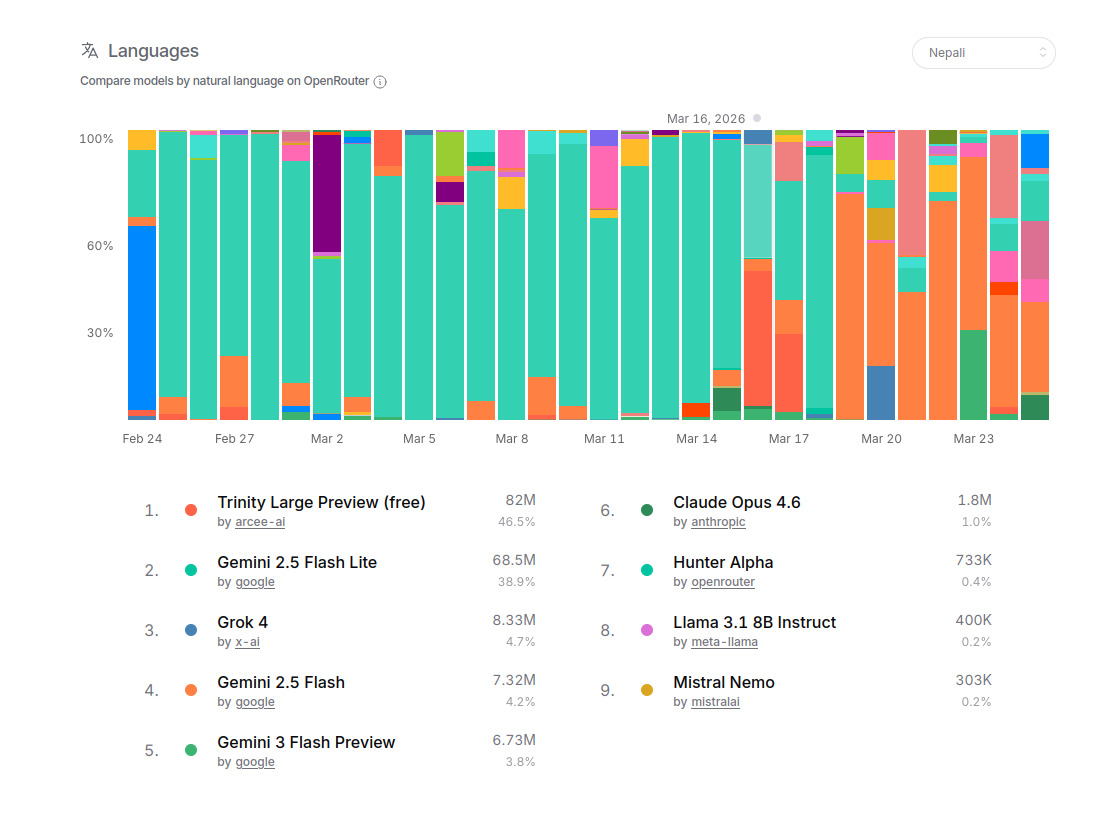
\includegraphics[width=\columnwidth]{trinity_openrouter.jpeg}
    \caption{Model usage share and token volume for the Nepali language on OpenRouter.}
    \label{fig:trinity_openrouter}
\end{figure}

\end{document}

%%% Local Variables:
%%% mode: latex
%%% TeX-master: t
%%% End:
